\chapter{Diagramas circuito}
\label{ap:diagramas}

\begin{figure}[h]
	\centering
	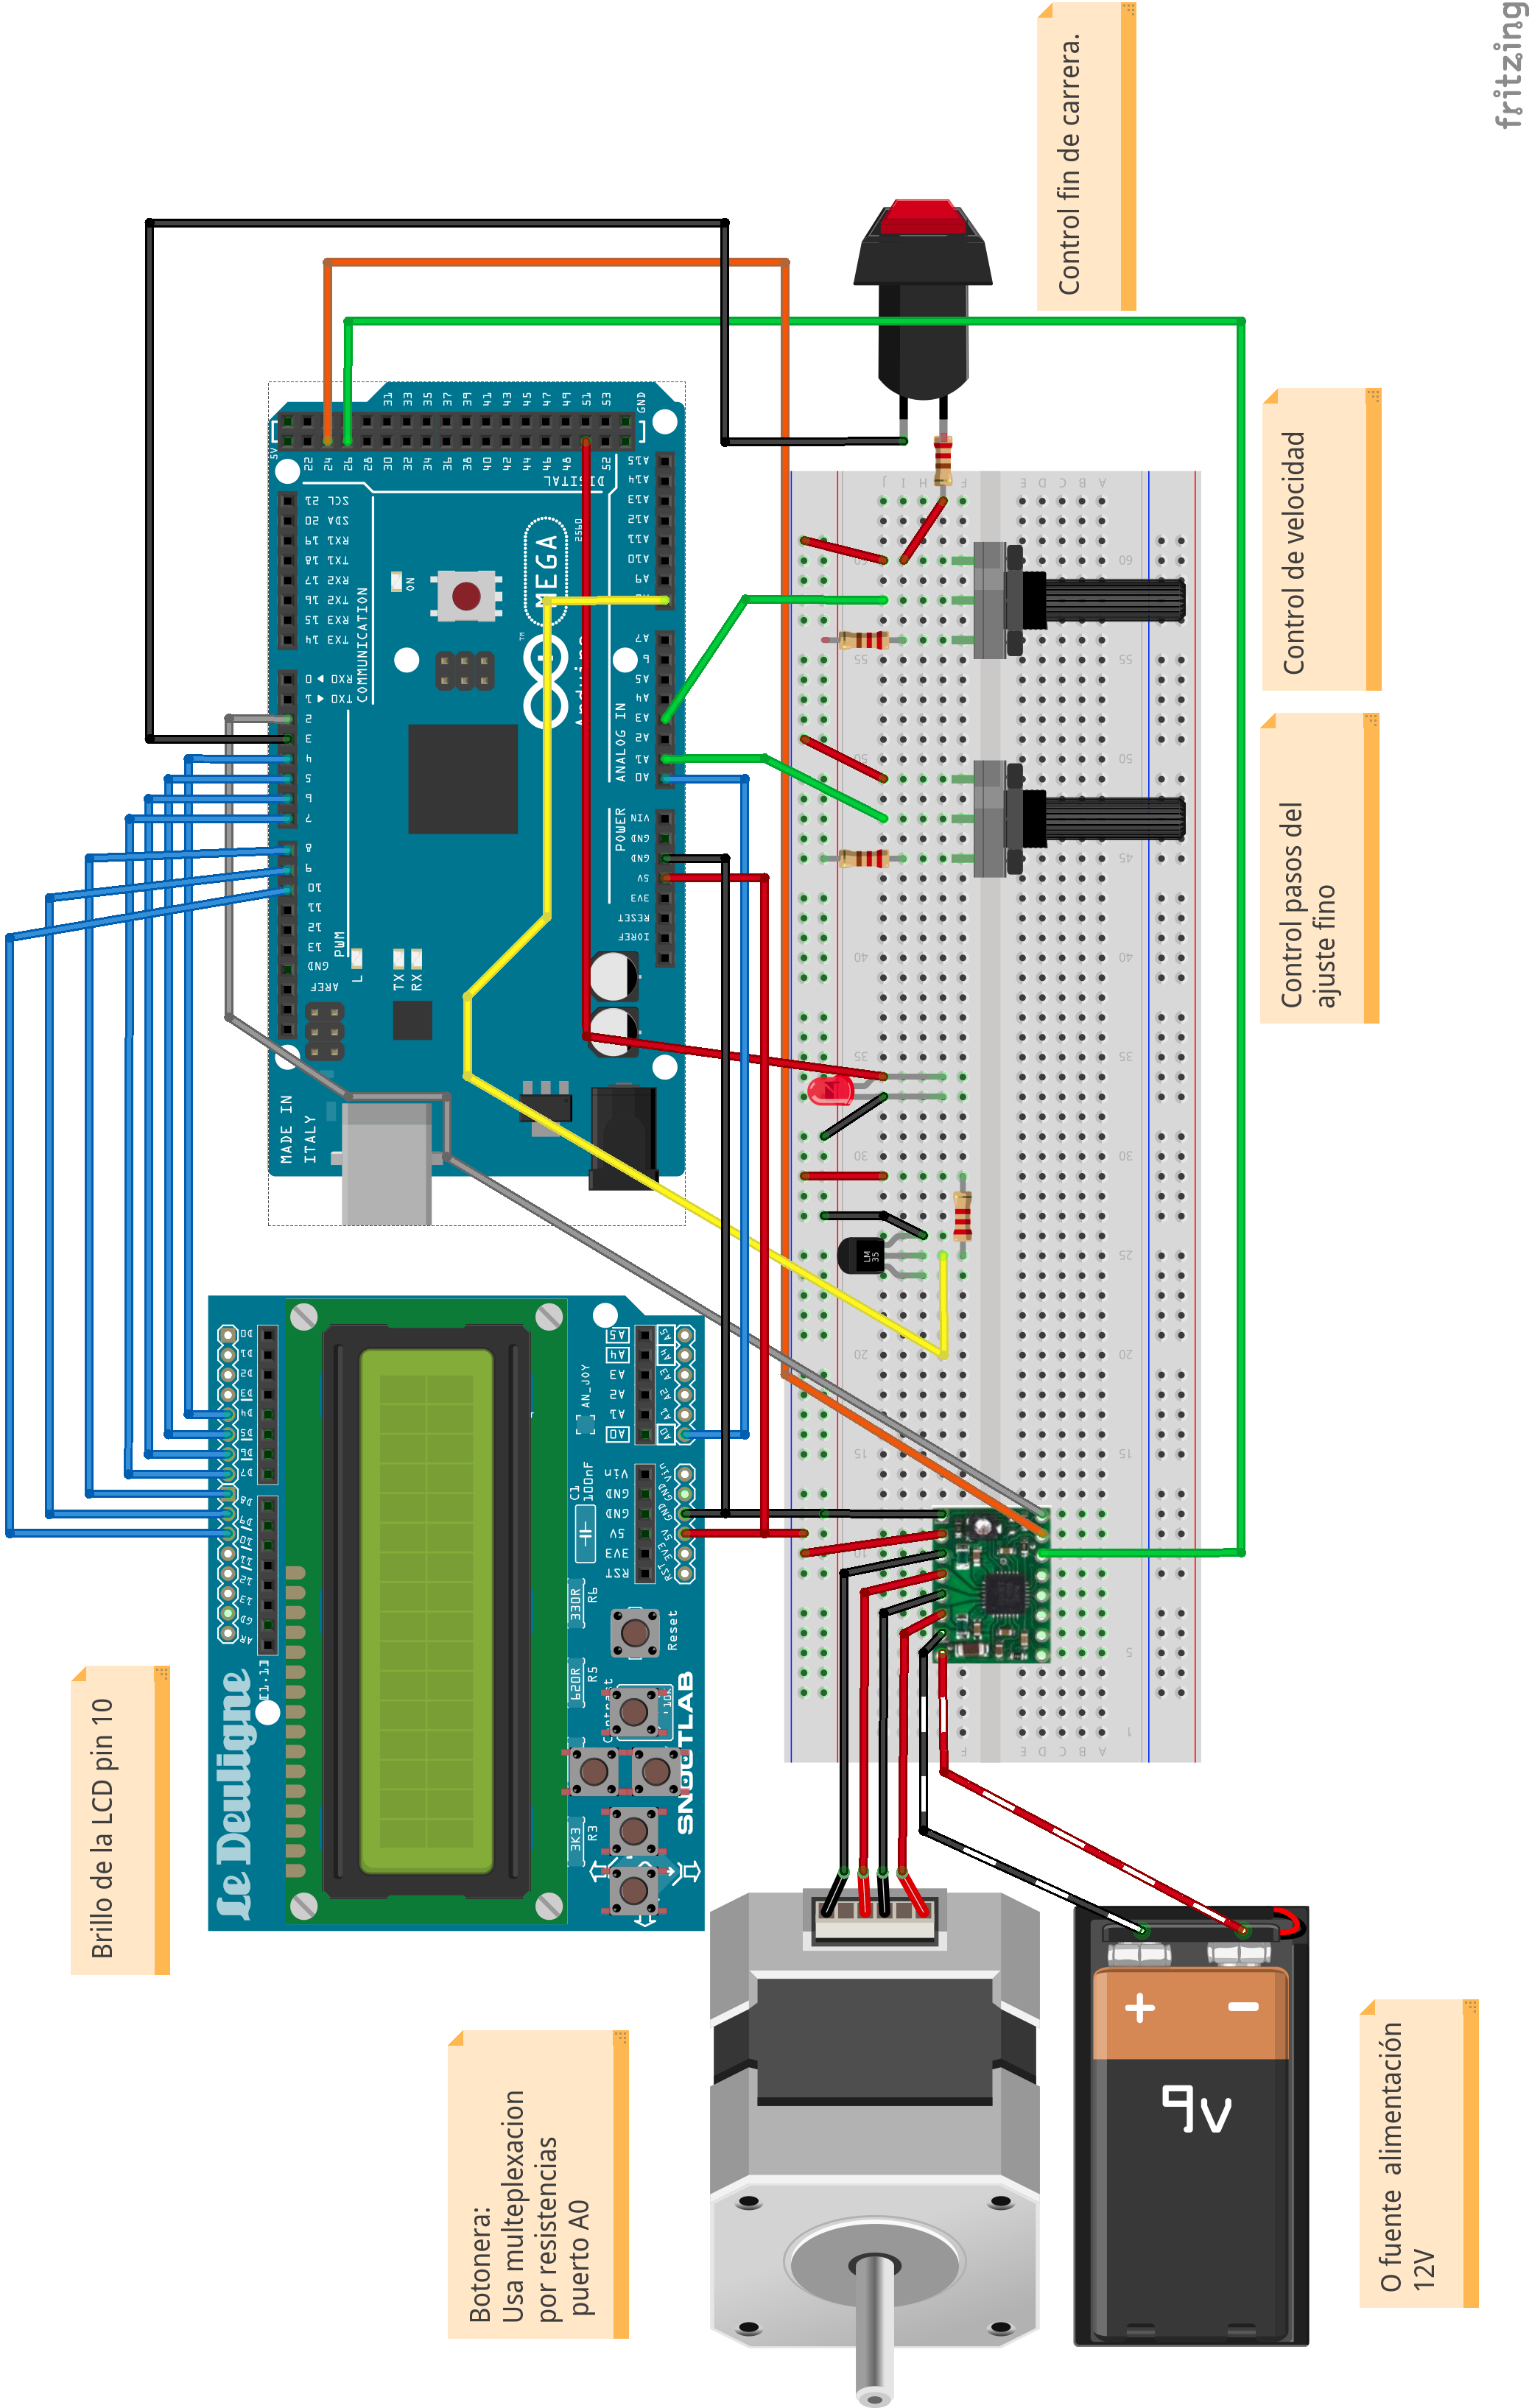
\includegraphics[width=1.0\textwidth]{../images/circuito1}
	\caption[Versión 0 del dispositivo]{Versión inicial del dispositivo, montado sobre una placa de prototipado, así como un módulo LCD con botonera y utilizando el controlador Arduino Mega.}
	\label{circuito1}
\end{figure}



\begin{figure}[h]
	\centering
	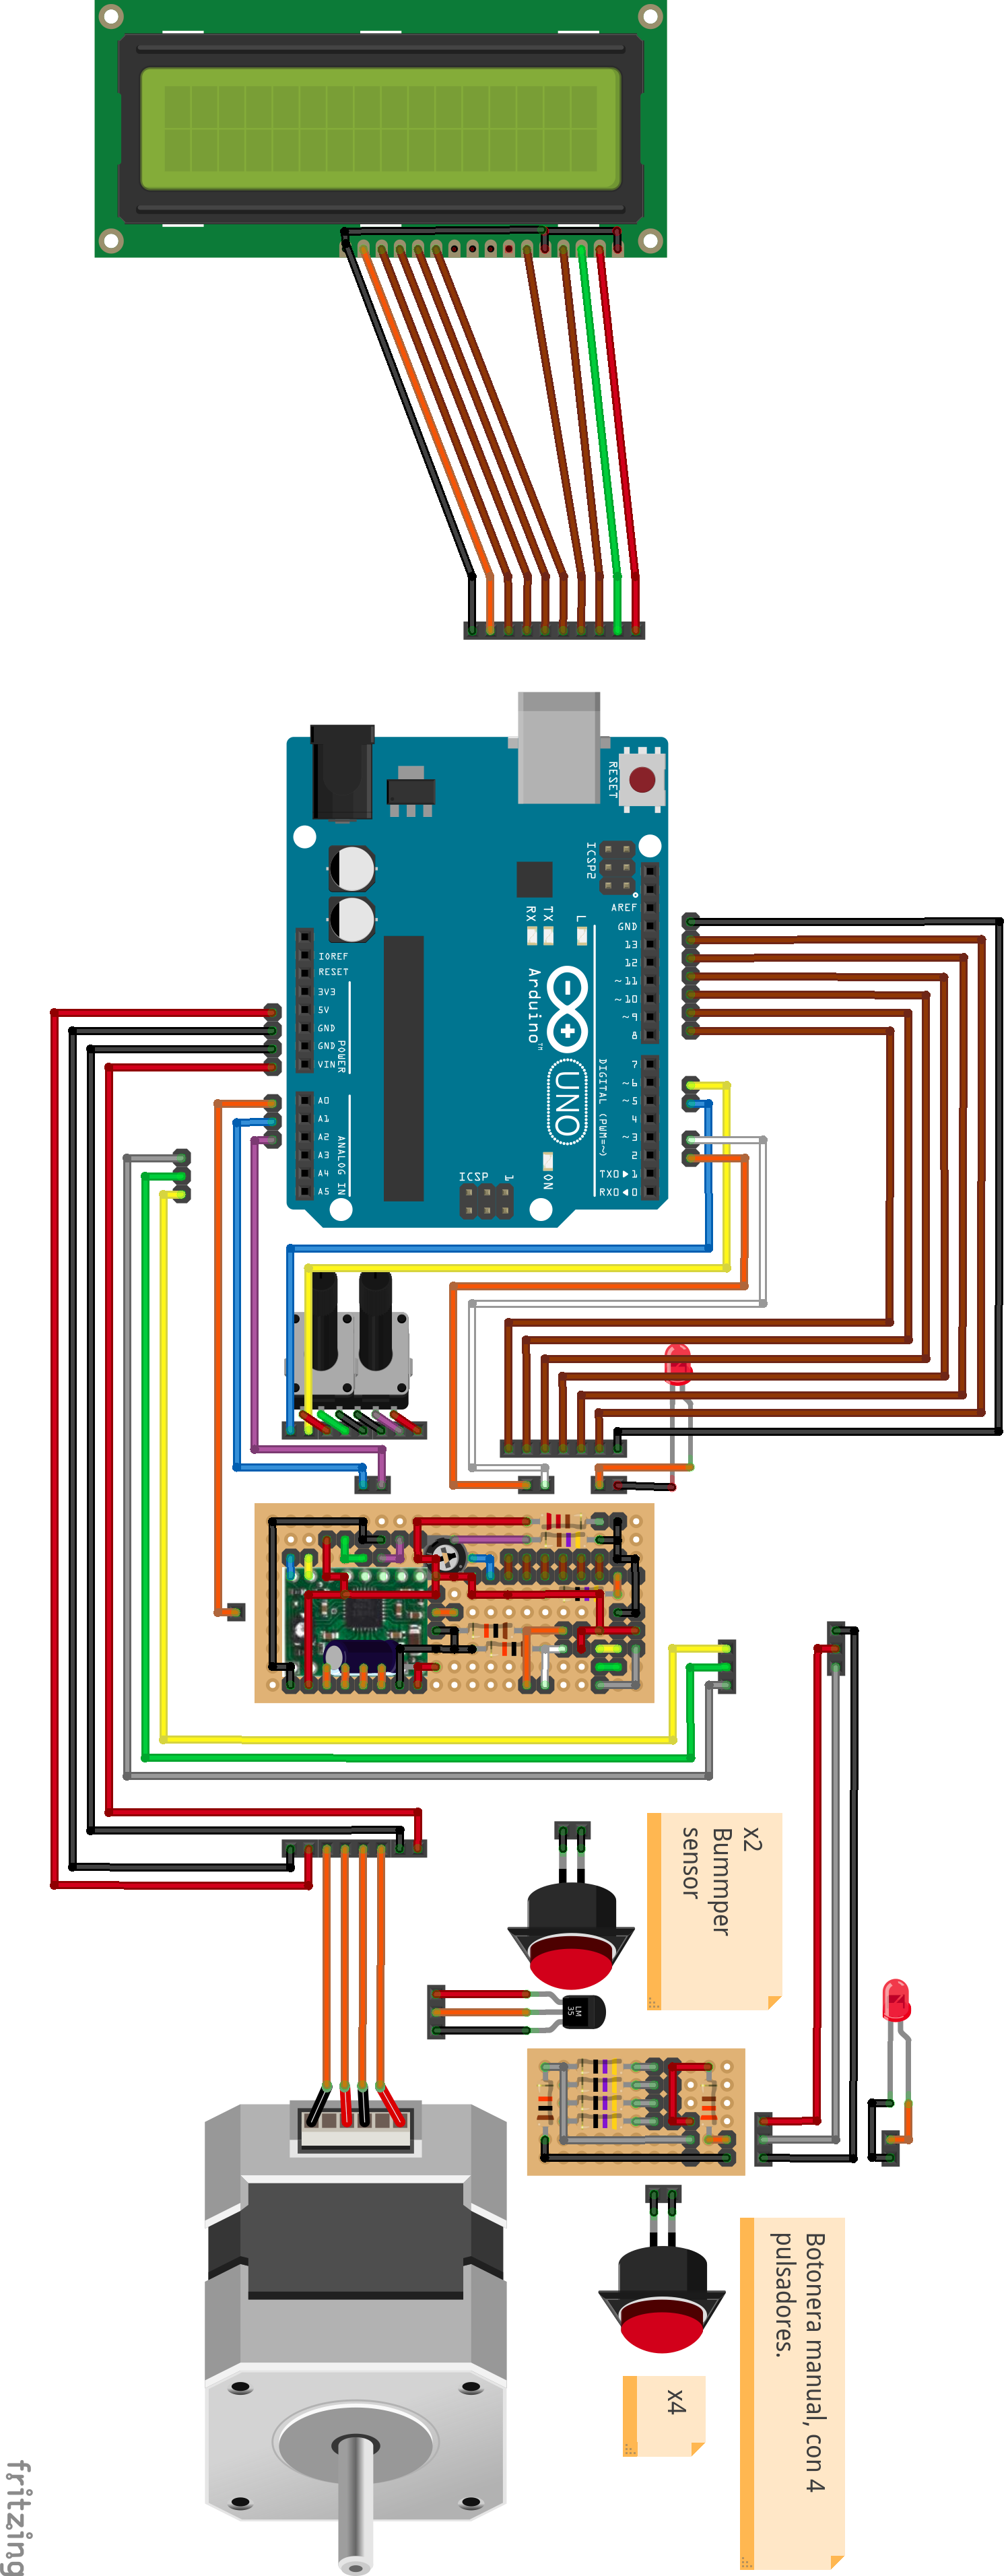
\includegraphics[width=0.65\textwidth]{../images/circuito2}
	\caption[Versión 1 del dispositivo]{Versión con pantalla LCD interfaz clásica, botonera analógica y Arduino UNO.}
	\label{circuito2}
\end{figure}


\begin{figure}[h]
	\centering
	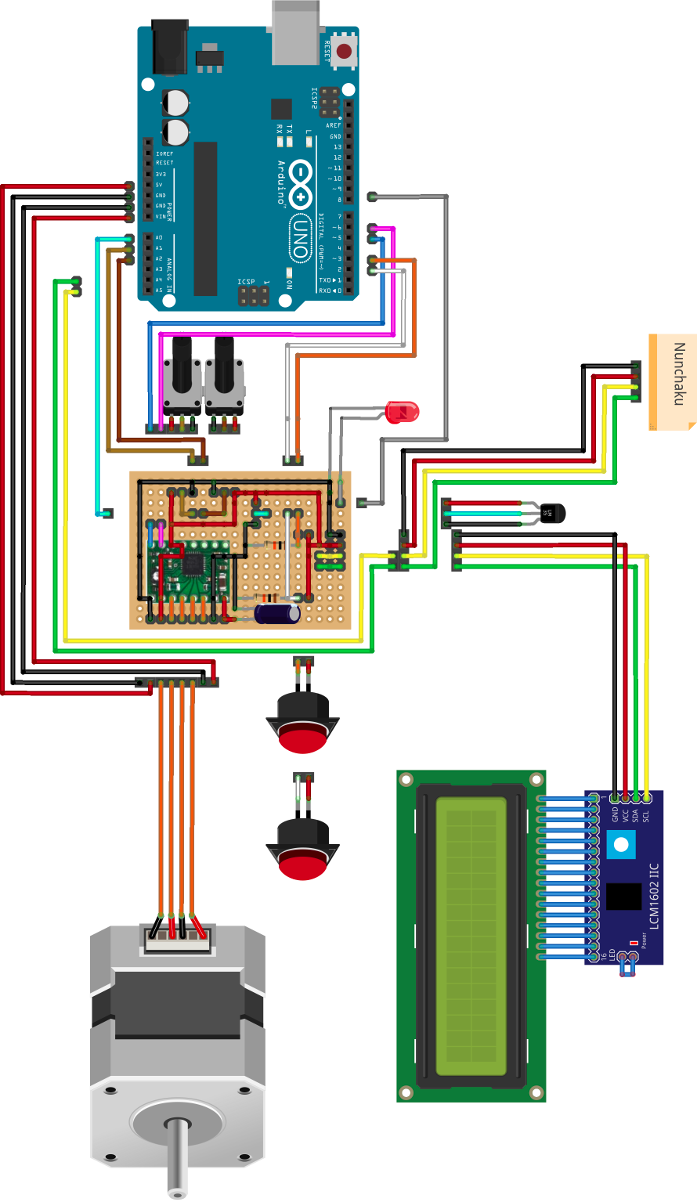
\includegraphics[width=0.9\textwidth]{../images/circuito3}
	\caption[Versión 2 del dispositivo]{Versión con pantalla LCD con interfaz I2C, mando Nunchuck, sensor de temperatura LM35 (interfaz analógico) y con controlador Arduino UNO.}
	\label{circuito3}
\end{figure}


\begin{figure}[h]
	\centering
	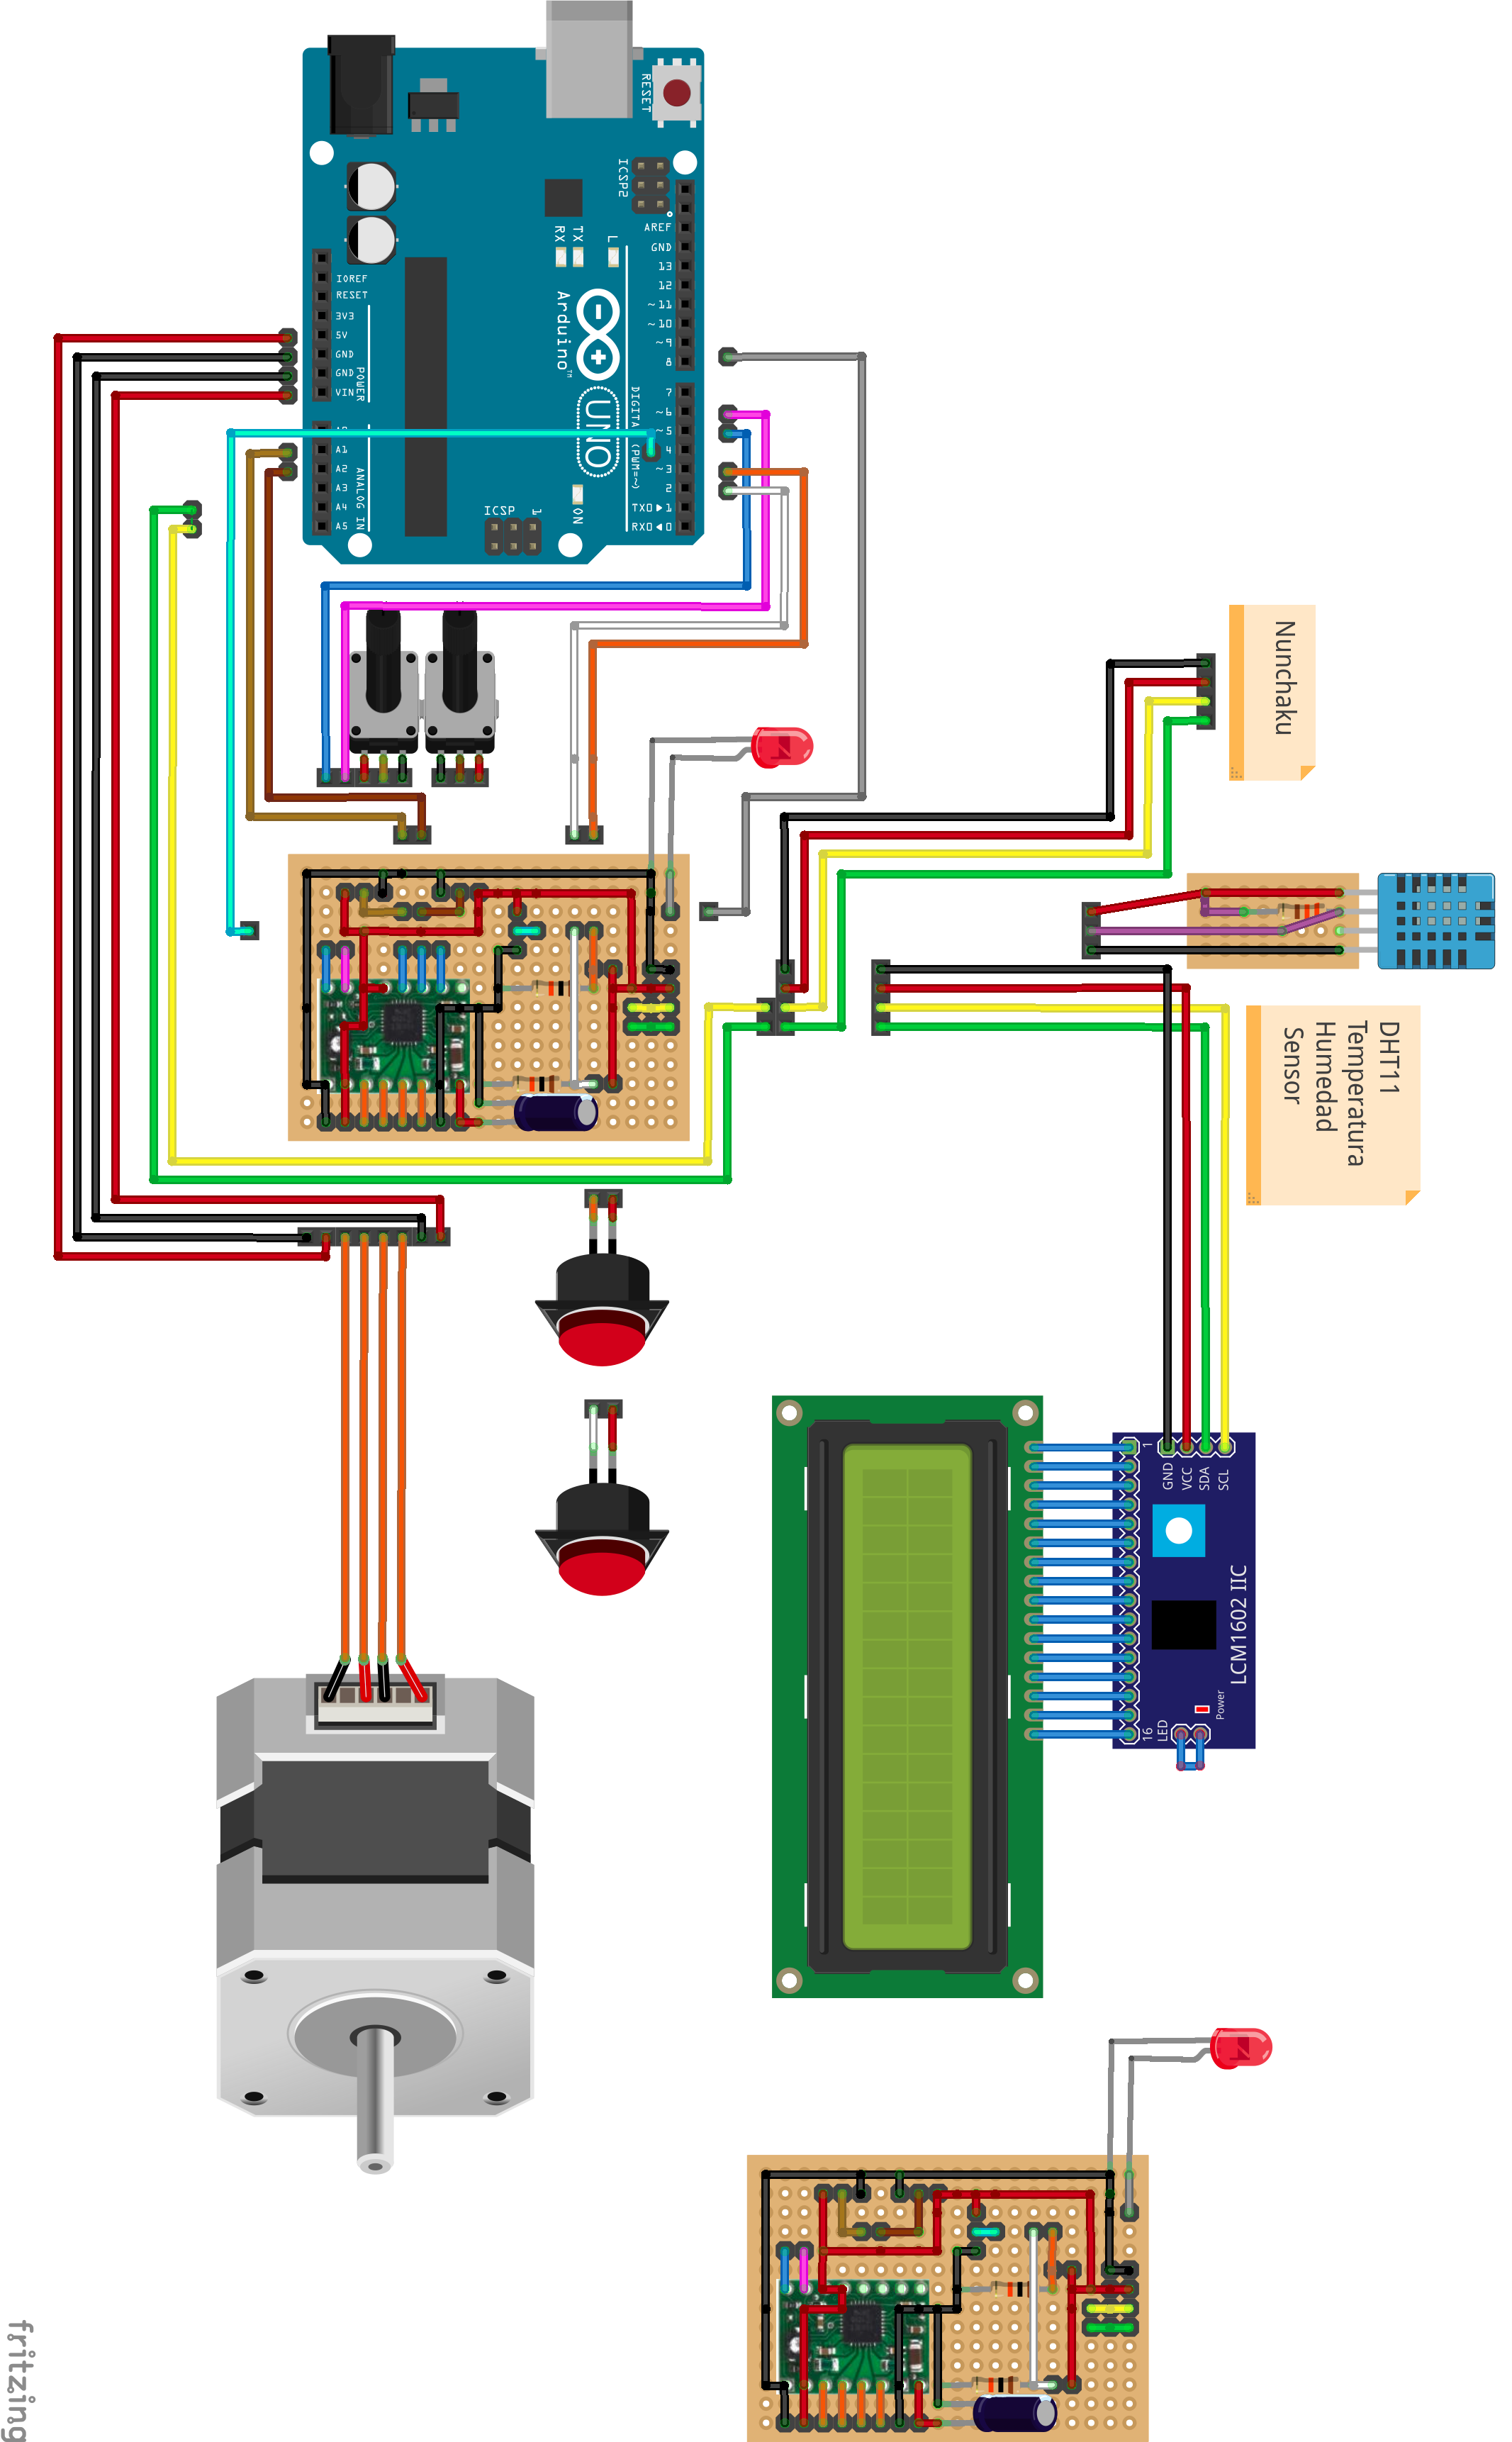
\includegraphics[width=0.9\textwidth]{../images/circuito4}
	\caption[Versión 3 del dispositivo]{Versión con pantalla LCD con interfaz I2C, mando Nunchuck, sensor de temperatura DHT11 (interfaz digital) ycon controlador Arduino UNO.}
	\label{circuito4}
\end{figure}






